\chapter{单变量函数}
前面中我们已经说明了如何由量的度量而产生实数
系。在这一章中我们要进一步说明如何用变数符号去表达变
量,用变数之间的函数关系去表达变量之间的关联。变数是
变量的抽象,函数是变量相互关系的抽象。在这一章里我们
还要运用极限来分析和确立连续函数的概念。

\section{函数的概念}
\subsection{变数和变域}
在研究自然现象时,人们会遇到许多不同的物理量,如
时间、长度、体积、速度、质量、力等等。按照给定条件,
能取许多不同数值的量叫做\textbf{变量};而只取一个数值的量叫做
\textbf{常量},用来表达变量的符号叫做\textbf{变数}。习惯上常用$x,y,
z$等字母表示变数,从纯数学的观点来说,一个变数就是一
个“能取许多不同数值”的符号,它所能取的所有数值构成
一个集合,叫做它的\textbf{变域}。如果变数$x$的变域已经给出,我
们就认为变数$x$是已知的。一般说来,任何数集可以当作变
数的变域。常会遇到取所有自然数的变数$n$, 譬如数列中的
项数。可是在现实生活中,我们通常研究的是连续变化的变
数,如动点所经过的路程及所花的时间等物理量,就是这种
变数的原形,数的区间就是这一类变数的变域,最常用的区
间是以两个实数$a$与$b$ $(a<b)$——它的两个端点——为界
限的有限区间,两个端点本身可以包含在区间内,也可以不
包含在内。因此我们可以把区间分为:
\begin{itemize}
    \item 开区间$(a,b)$就是$\{x|a<x<b\}$;
    \item  闭区间$[a,b]$就是$\{x|a\le x\le b\}$;
    \item  半开区间$(a,b]$就是$\{x|a<x\le b\}$;
    $[a,b)$就是$\{x|a\le x<b\}$。
\end{itemize}
在上述各种情形,数$b-a$为区间的长度。

常量可以看作变量的特殊情形,它的变域是由一个数组
成的集合$\{x|x=a\}$。

数轴上的线段是数的区间的几何表示,图示开区间如图
8.1或8.2。

在点$a,b$处的圆圈或圆括号表示从区间去掉这两个
数。在两个圆圈之间的粗线段表示在$a,b$之间的一切数$x$。
图示闭区间如图8.3。
图示半开区间如图8.4、8.5,每一种情形都只包含出现
有方括号的数,以及在$a,b$之间的一切实数。
\begin{figure}[htp]\centering
    \begin{minipage}[t]{0.48\textwidth}
    \centering
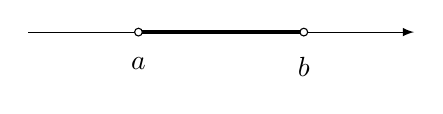
\begin{tikzpicture}[>=latex, scale=.7]
       \draw[->] (0.5,0)--(7.5,0);
       \draw[ultra thick] (2.5,0)node[below=5pt]{$a$}--(5.5,0)node[below=5pt]{$b$};
       \draw (2.5,0)[fill=white] circle (2pt);
        \draw (5.5,0)[fill=white] circle (2pt);
    \end{tikzpicture}
    \caption{}
    \end{minipage}
    \begin{minipage}[t]{0.48\textwidth}
    \centering
    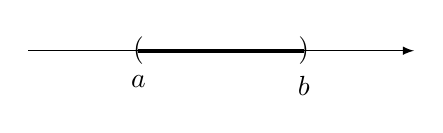
\begin{tikzpicture}[>=latex, scale=.7]
        \draw[->] (0.5,0)--(7.5,0);
        \draw[ultra thick] (2.5,0)node[below=5pt]{$a$}--(5.5,0)node[below=5pt]{$b$};
        \node at (2.5,0){$($}; \node at (5.5,0){$)$};
    \end{tikzpicture}
    \caption{}
    \end{minipage}
    \end{figure}

\begin{figure}[htp]\centering
    \begin{minipage}[t]{0.48\textwidth}
    \centering
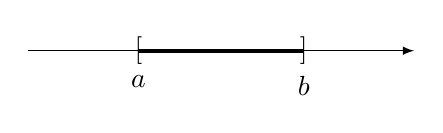
\begin{tikzpicture}[>=latex, scale=.7]
    \draw[->] (0.5,0)--(7.5,0);
    \draw[ultra thick] (2.5,0)node[below=5pt]{$a$}--(5.5,0)node[below=5pt]{$b$};
    \node at (2.5,0){$[$}; \node at (5.5,0){$]$};
    \end{tikzpicture}
    \caption{}
    \end{minipage}
    \begin{minipage}[t]{0.48\textwidth}
    \centering
    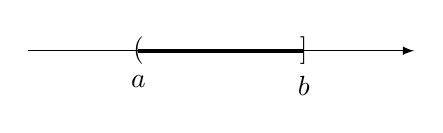
\begin{tikzpicture}[>=latex, scale=.7]
        \draw[->] (0.5,0)--(7.5,0);
        \draw[ultra thick] (2.5,0)node[below=5pt]{$a$}--(5.5,0)node[below=5pt]{$b$};
        \node at (2.5,0){$($}; \node at (5.5,0){$]$};
    \end{tikzpicture}
    \caption{}
    \end{minipage}
    \end{figure}

\begin{figure}[htp]\centering
    \begin{minipage}[t]{0.48\textwidth}
    \centering
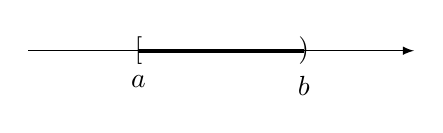
\begin{tikzpicture}[>=latex, scale=.7]
    \draw[->] (0.5,0)--(7.5,0);
    \draw[ultra thick] (2.5,0)node[below=5pt]{$a$}--(5.5,0)node[below=5pt]{$b$};
    \node at (2.5,0){$[$}; \node at (5.5,0){$)$};
    \end{tikzpicture}
    \caption{}
    \end{minipage}
    \begin{minipage}[t]{0.48\textwidth}
    \centering
    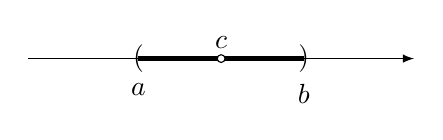
\begin{tikzpicture}[>=latex, scale=.7]
        \draw[->] (0.5,0)--(7.5,0);
        \draw[ultra thick] (2.5,0)node[below=5pt]{$a$}--(5.5,0)node[below=5pt]{$b$};
        \node at (2.5,0){$($}; \node at (5.5,0){$)$};
        \draw (4,0)[fill=white] circle (2pt)node[above]{$c$};
    \end{tikzpicture}
    \caption{}
    \end{minipage}
    \end{figure}

有时也要考虑无穷区间,用符号$-\infty,+\infty$作为一端或
两端,它们的记号和上面所引进的相类似,例如$(-\infty,+\infty)$
是全体实数集合$\{x|x\in\mathbb{R}\}$, 区间$(a,+\infty)$表示集
合$\{x|x>a\}$, 区间$(-\infty,b]$表示集合$\{x|x\le b\}$. 无穷区间
在几何上可用两端无限伸延的直线或一端无限伸延的射线来
表示。

以后我们要常用到一点的邻域的概念。\textbf{$c$点的邻域}是包
含$c$点的任何开区间$(a,b)$, 而$c$点的去心邻域指去掉$c$
点的任何$c$点的邻域。它的图象如图8.6。

$c$点的去心邻域可写成$(a,c)\cup (c,b)$. 我们常把
$c$点的邻域写成对称的形式:$(c-r,c+r)$, 对任何
$r>0$, 并且称它为\textbf{$c$点的对称邻域}。









